\begin{center}
  \textbf{Отчёт лабораторной работы №\envReportLabNumber}
\end{center}

\textbf{Тема}:
<<\envReportTitle>>

\textbf{Цель}:
изучить основы методов Text Mining (текстовой добычи), приобрести
навыки работы с методами Text Mining (текстовой добычи) в системе
STATISTICA StatSoft, осуществить обработку методами Text Mining
индивидуального набора данных и интерпретацию результатов.
% = = = = = = = = = = = = = = = =

\begin{center}
  \textbf{Ход работы}
\end{center}

Удаляю папку <<Statistica 10 RUS>> (тут временные файлы portable программы).

Запускаю Ststatistica\_10\_ru\_portable.exe.

\begin{center}
  \textbf{Определение анализа}
\end{center}

Главная > Открыть > Reuters3000.sta  > Открыть

Результаты на рисунке~\ref{fig:1}.

\begin{figure}[!h]
  \centering

  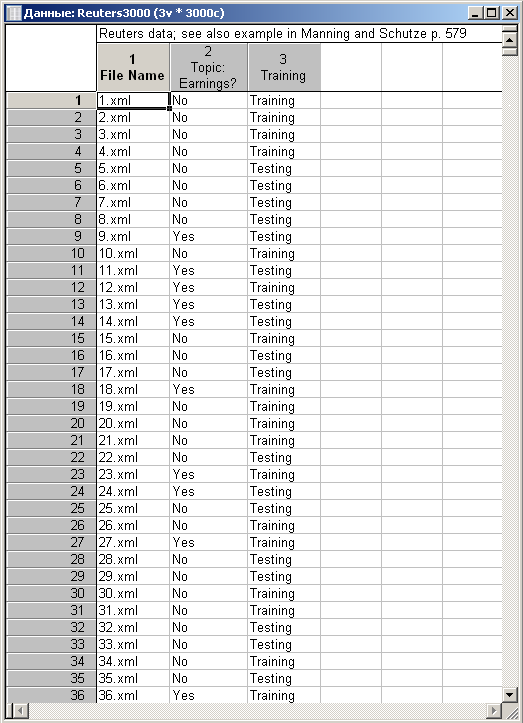
\includegraphics[height=14cm]
  {inc/1.PNG}

  \caption{1}

  \label{fig:1}
\end{figure}

\newpage

Добыча Данных > Добыча текста > Quick \\
> Retrieve text from: > Files > Paths in spreadsheet > Document paths \\
> 1 – File Name > OK \\

Результаты на рисункax~\ref{fig:2}, \ref{fig:3}, \ref{fig:4}.

\begin{figure}[!h]
  \centering

  \begin{minipage}{0.32\textwidth}
    \centering

    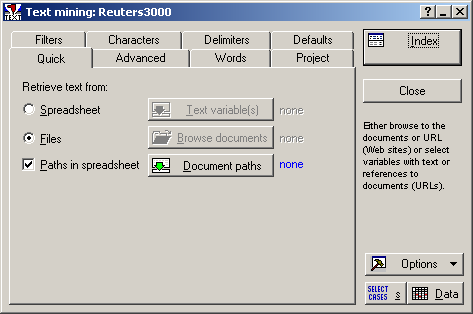
\includegraphics[height=4cm]
    {inc/2.PNG}

    \caption{2}

    \label{fig:2}
  \end{minipage}
  \begin{minipage}{0.32\textwidth}
    \centering

    \includegraphics[height=4cm]
    {inc/3.PNG}

    \caption{3}

    \label{fig:3}
  \end{minipage}
  \begin{minipage}{0.32\textwidth}
    \centering

    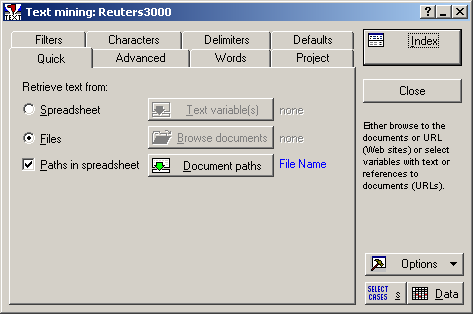
\includegraphics[height=4cm]
    {inc/4.PNG}

    \caption{4}

    \label{fig:4}
  \end{minipage}
\end{figure}

> Advanced > Stemming language > English \\
> \% files where word occurs: > Min > 3 \\
> Words > Stop words (discarded, excluded from indexing) > Select > EnglishStopList,txt > Открыть \\

Результаты на рисункax~\ref{fig:5}, \ref{fig:6}, \ref{fig:7}, \ref{fig:8}.

\begin{figure}[!h]
  \centering

  \begin{minipage}{0.49\textwidth}
    \centering

    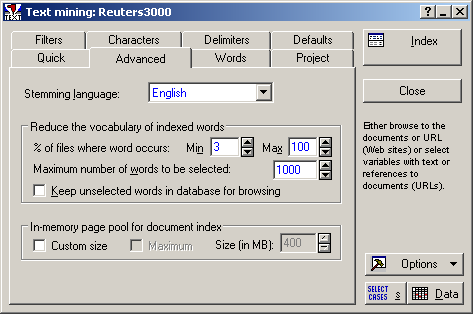
\includegraphics[height=5cm]
    {inc/5.PNG}

    \caption{5}

    \label{fig:5}
  \end{minipage}
  \begin{minipage}{0.49\textwidth}
    \centering

    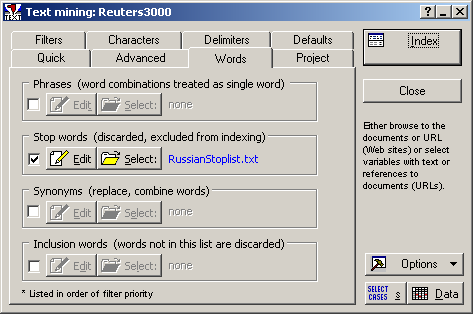
\includegraphics[height=5cm]
    {inc/6.PNG}

    \caption{6}

    \label{fig:6}
  \end{minipage}
\end{figure}

\begin{figure}[!h]
  \centering

  \begin{minipage}{0.49\textwidth}
    \centering

    \includegraphics[height=5cm]
    {inc/7.PNG}

    \caption{7}

    \label{fig:7}
  \end{minipage}
  \begin{minipage}{0.49\textwidth}
    \centering

    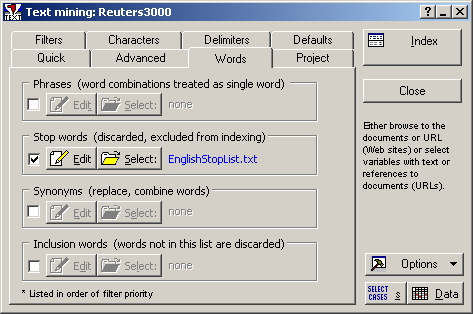
\includegraphics[height=5cm]
    {inc/8.PNG}

    \caption{8}

    \label{fig:8}
  \end{minipage}
\end{figure}

\newpage

\begin{center}
  \textbf{Выполнение анализа данных}
\end{center}

> Index > Да

Результаты на рисунке~\ref{fig:9}.

\begin{figure}[!h]
  \centering

  \includegraphics[height=2cm]
  {inc/9.PNG}

  \caption{9}

  \label{fig:9}
\end{figure}

\begin{center}
  \textbf{Сохранения извлеченных частот слов во входной файл}
\end{center}

> Save results > Ammount > 342 > Append empty variables > OK \\
> Save results > Write back current results (to selected variables) \\

Результаты на рисункax~\ref{fig:10}, \ref{fig:11}, \ref{fig:12}.

\begin{figure}[!h]
  \centering

  \begin{minipage}{0.49\textwidth}
    \centering

    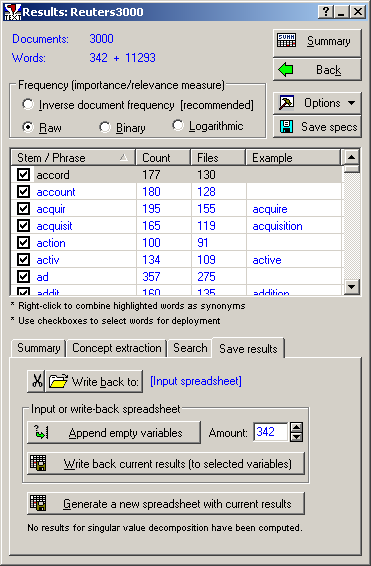
\includegraphics[height=7cm]
    {inc/10.PNG}

    \caption{10}

    \label{fig:10}
  \end{minipage}
  \begin{minipage}{0.49\textwidth}
    \centering

    \includegraphics[height=2cm]
    {inc/11.PNG}

    \caption{11}

    \label{fig:11}
  \end{minipage}
\end{figure}

\begin{figure}[p!h]
  \centering

  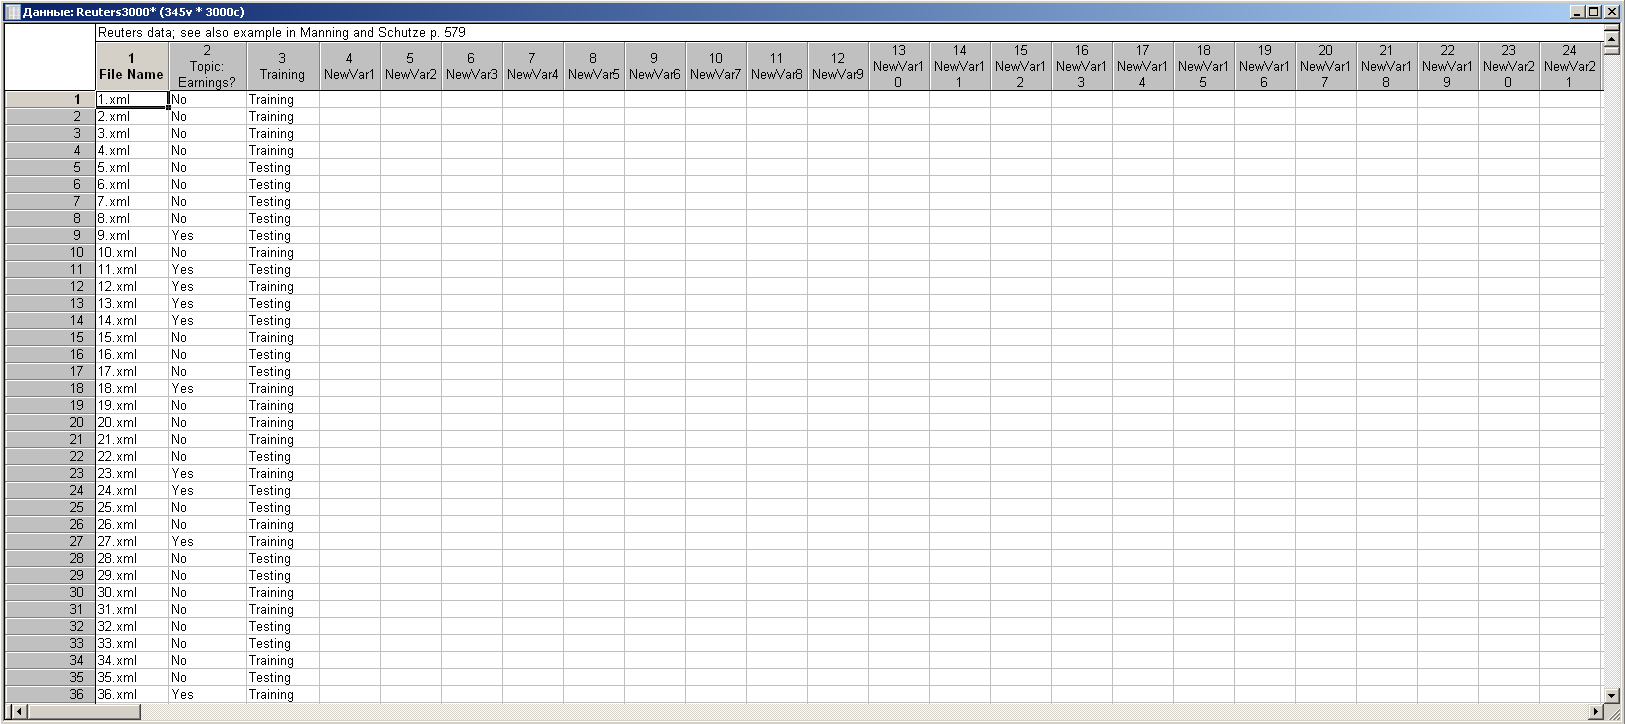
\includegraphics[width=17cm]
  {inc/12.PNG}

  \caption{12}

  \label{fig:12}
\end{figure}

> Statistics > account > Shift > york \\
> Variables > 4 - NewVar1 > Shift > 345 — NewVar342 \\
> Присвоить > OK \\

Результаты на рисункax~\ref{fig:13}, \ref{fig:14}, \ref{fig:15}.

\begin{figure}[p!h]
  \centering

  \begin{minipage}{0.49\textwidth}
    \centering

    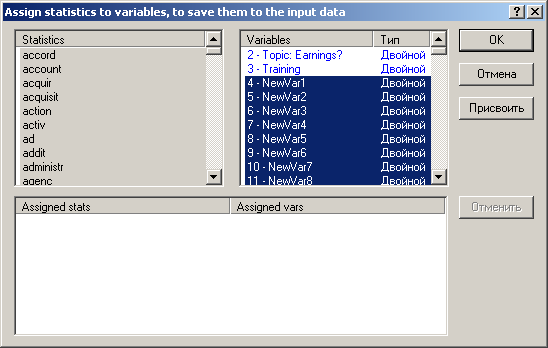
\includegraphics[height=5cm]
    {inc/13.PNG}

    \caption{13}

    \label{fig:13}
  \end{minipage}
  \begin{minipage}{0.49\textwidth}
    \centering

    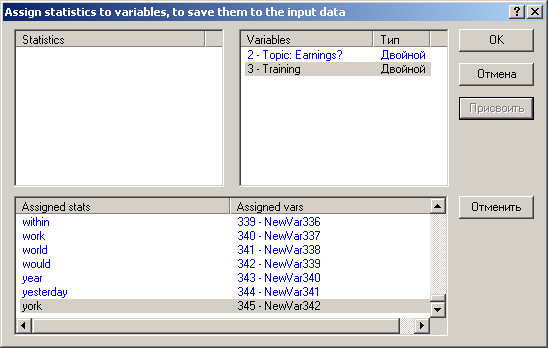
\includegraphics[height=5cm]
    {inc/14.PNG}

    \caption{14}

    \label{fig:14}
  \end{minipage}
\end{figure}

\begin{figure}[p!h]
  \centering

  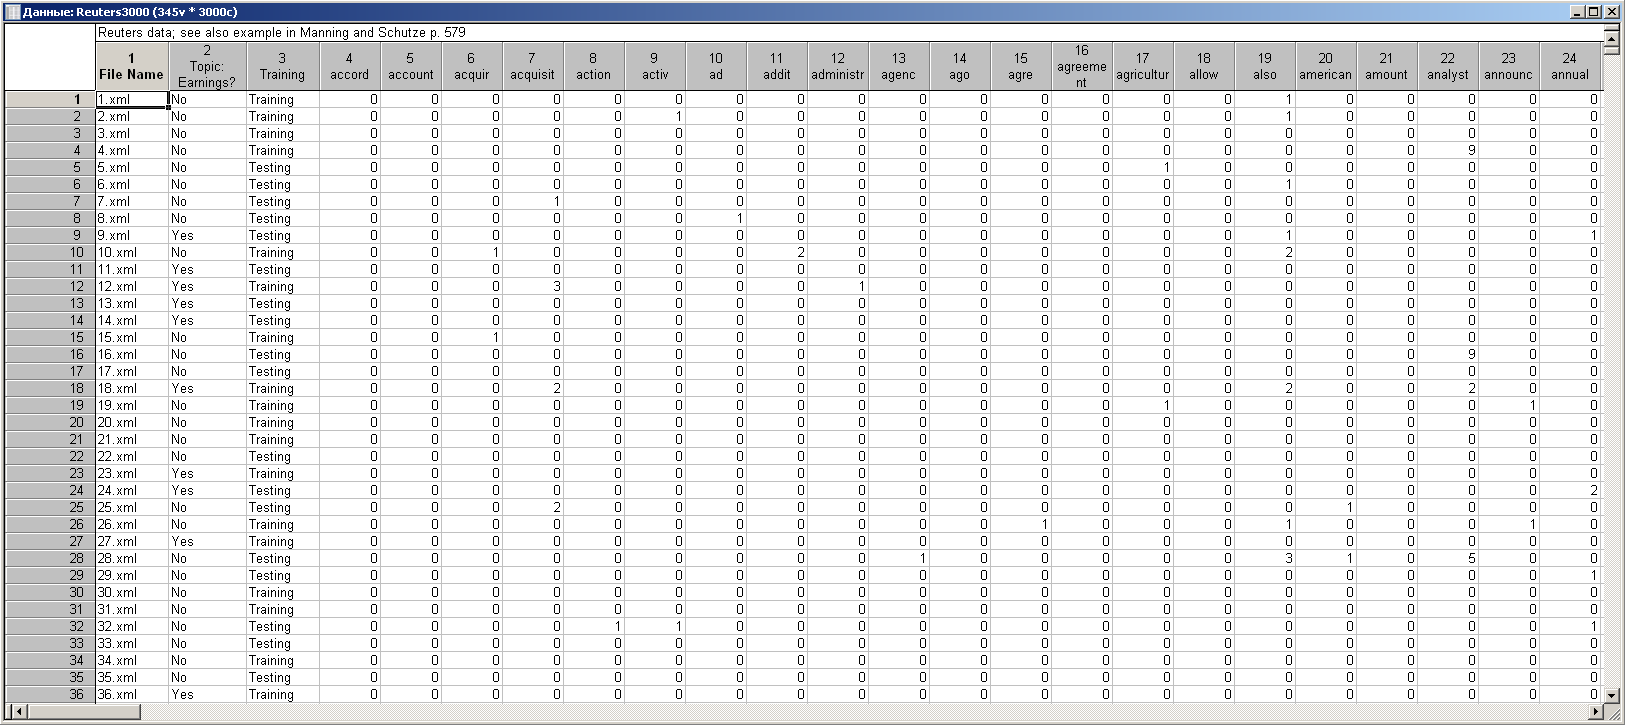
\includegraphics[width=17cm]
  {inc/15.PNG}

  \caption{15}

  \label{fig:15}
\end{figure}

\newpage

\begin{center}
  \textbf{Первоначальный выбор функций}
\end{center}

> Добыча Данных > Отсеивание признаков > Variables \\
> Dependent, categorical > 2 — Topic: Earnings \\
> Predictors; contimuous > 4 — accord > Shift > 345-york \\
> OK > OK \\

Результаты на рисункax~\ref{fig:16}, \ref{fig:17}, \ref{fig:18}.

\begin{figure}[!h]
  \centering

  \begin{minipage}{0.22\textwidth}
    \centering

    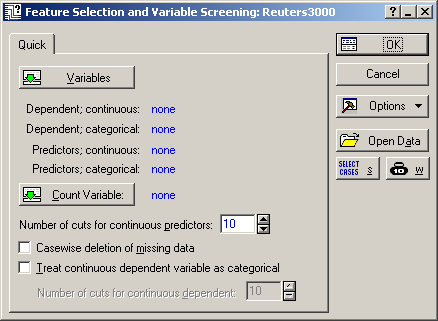
\includegraphics[height=3cm]
    {inc/16.PNG}

    \caption{16}

    \label{fig:16}
  \end{minipage}
  \begin{minipage}{0.52\textwidth}
    \centering

    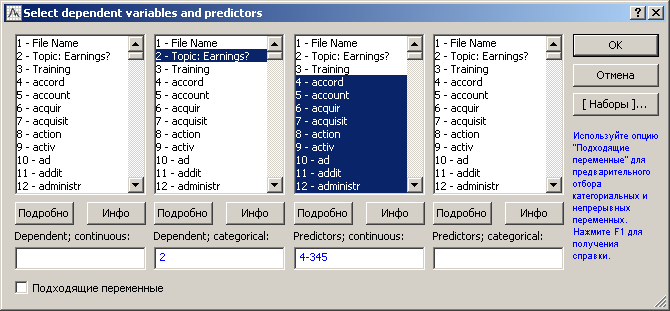
\includegraphics[height=4cm]
    {inc/17.PNG}

    \caption{17}

    \label{fig:17}
  \end{minipage}
  \begin{minipage}{0.22\textwidth}
    \centering

    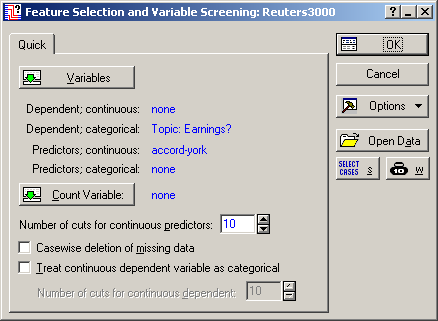
\includegraphics[height=3cm]
    {inc/18.PNG}

    \caption{18}

    \label{fig:18}
  \end{minipage}
\end{figure}

> Quick > Display > 50 > Histogram of importance for best k predictors \\

Результаты на рисункax~\ref{fig:19}, \ref{fig:20}.

\begin{figure}[!h]
  \centering

  \begin{minipage}{0.29\textwidth}
    \centering

    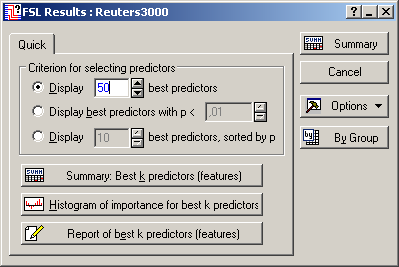
\includegraphics[height=4cm]
    {inc/19.PNG}

    \caption{19}

    \label{fig:19}
  \end{minipage}
  \begin{minipage}{0.69\textwidth}
    \centering

    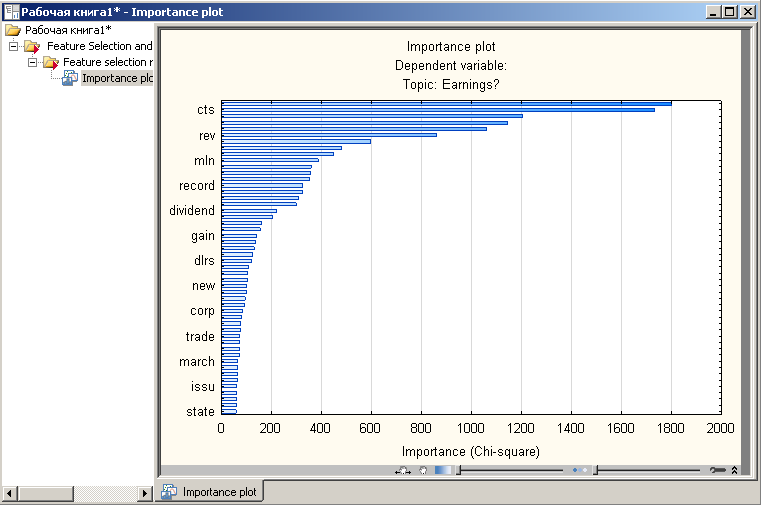
\includegraphics[height=6cm]
    {inc/20.PNG}

    \caption{20}

    \label{fig:20}
  \end{minipage}
\end{figure}

FSL Results L Reuters3000 > Quick > Display > 20 \\
> Histogram of importance for best k predictors

Результаты на рисункax~\ref{fig:21}, \ref{fig:22}.

\begin{figure}[!h]
  \centering

  \begin{minipage}{0.29\textwidth}
    \centering

    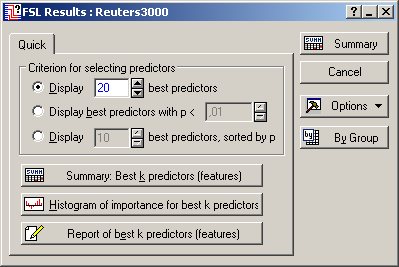
\includegraphics[height=4cm]
    {inc/21.PNG}

    \caption{21}

    \label{fig:21}
  \end{minipage}
  \begin{minipage}{0.69\textwidth}
    \centering

    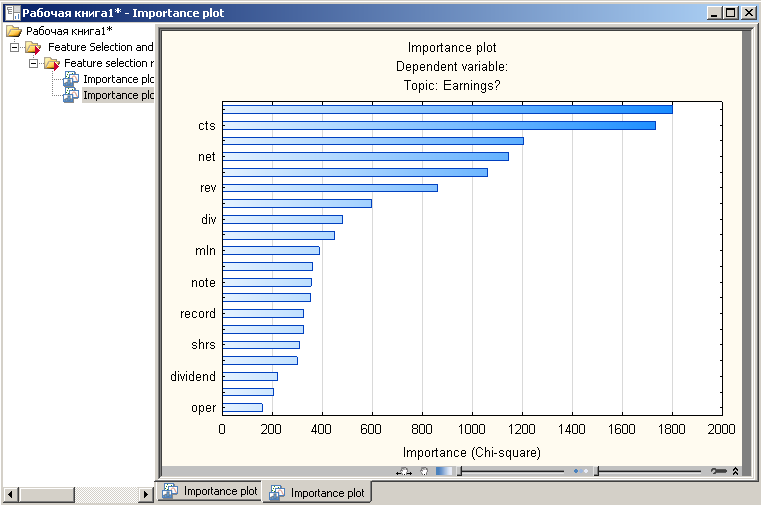
\includegraphics[height=6cm]
    {inc/22.PNG}

    \caption{22}

    \label{fig:22}
  \end{minipage}
\end{figure}

\newpage

FSL Results L Reuters3000 > Quick > Display > 20 \\
> Report of best k predictors (features) \\

Результаты на рисунке~\ref{fig:23}.

Копируем номера переменных:
332 86 296 207 280 274 182 102 248 197 242 212 255 263 256 297 35 103 338 221

\begin{figure}[!h]
  \centering

  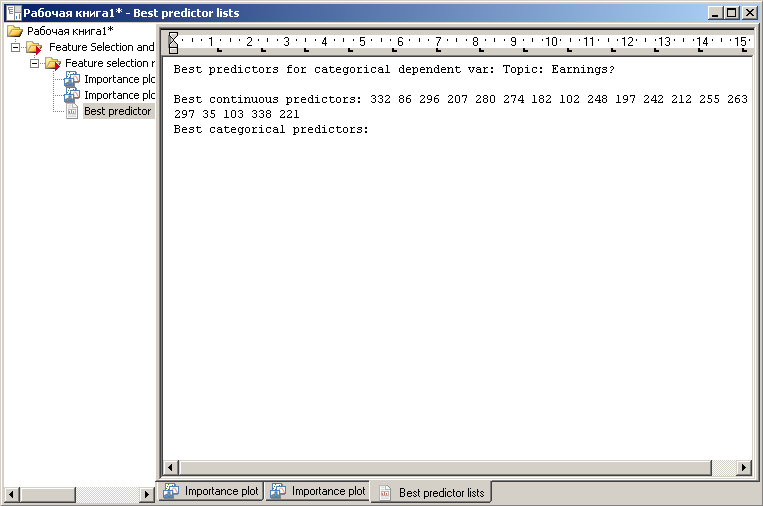
\includegraphics[height=6cm]
  {inc/23.PNG}

  \caption{23}

  \label{fig:23}
\end{figure}

Вид > Класическое Меню \\
> Добыча Данных > Общие деревья классификаии и регрессии \\
> Quick \\
> Type of analysis > Standart C\&RT \\
> Specification method > Quick specs dialog \\
> OK \\

Результат на рисунке~\ref{fig:24}.

\begin{figure}[!h]
  \centering

  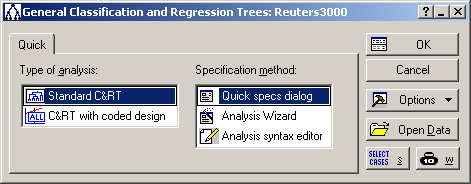
\includegraphics[height=4cm]
  {inc/24.PNG}

  \caption{24}

  \label{fig:24}
\end{figure}

\newpage

> Quick > Categorical response (categorical dependent variable) (checked) \\
> Variables \\
> Depend > 2 — Topic: \\
> Continuous pred\\
> 332 86 296 207 280 274 182 102 248 197 242 212 255 263 256 297 35 103 338 221 > OK\\

Результаты на рисункax~\ref{fig:25}, \ref{fig:26}.

\begin{figure}[!h]
  \centering

  \begin{minipage}{0.29\textwidth}
    \centering

    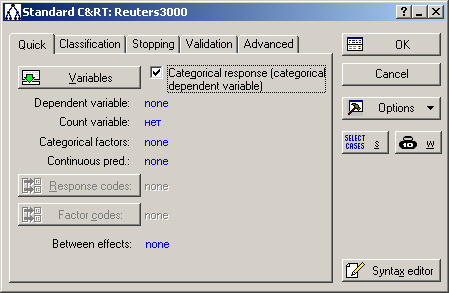
\includegraphics[height=4cm]
    {inc/25.PNG}

    \caption{25}

    \label{fig:25}
  \end{minipage}
  \begin{minipage}{0.69\textwidth}
    \centering

    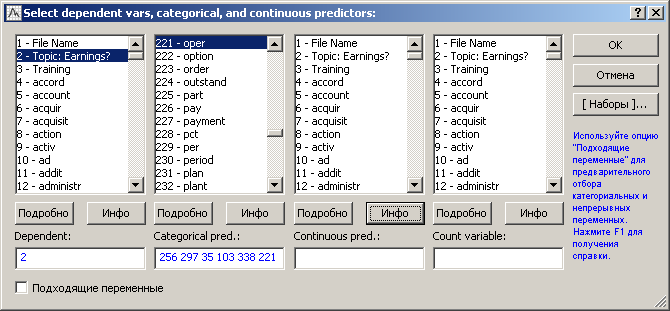
\includegraphics[height=4.5cm]
    {inc/26.PNG}

    \caption{26}

    \label{fig:26}
  \end{minipage}
\end{figure}

> Validation > V-fold cross-validation \\
> Test sample \\
> Status > on \\
> Sample Identifier Variable > 3 — Training > OK \\
> OK > OK \\

Результаты на рисункax~\ref{fig:27}, \ref{fig:28}, \ref{fig:29}, \ref{fig:30}.

\begin{figure}[!h]
  \centering

  \begin{minipage}{0.49\textwidth}
    \centering

    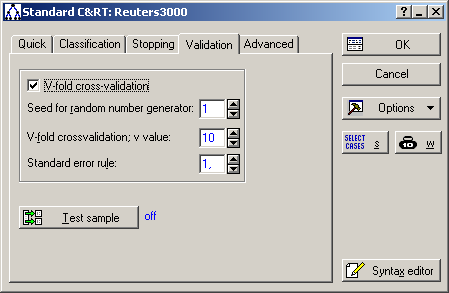
\includegraphics[height=4cm]
    {inc/27.PNG}

    \caption{27}

    \label{fig:27}
  \end{minipage}
  \begin{minipage}{0.49\textwidth}
    \centering

    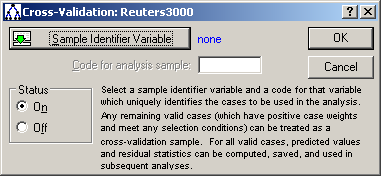
\includegraphics[height=4cm]
    {inc/28.PNG}

    \caption{28}

    \label{fig:28}
  \end{minipage}
\end{figure}

\begin{figure}[!h]
  \centering

  \begin{minipage}{0.49\textwidth}
    \centering

    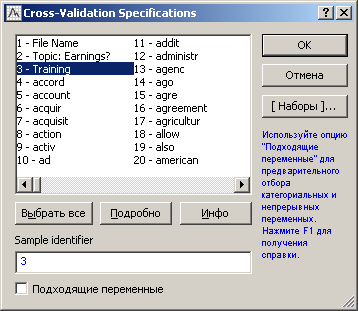
\includegraphics[height=4cm]
    {inc/29.PNG}

    \caption{29}

    \label{fig:29}
  \end{minipage}
  \begin{minipage}{0.49\textwidth}
    \centering

    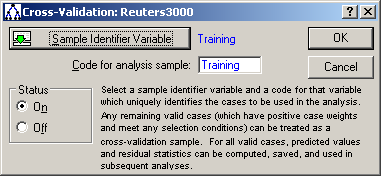
\includegraphics[height=4cm]
    {inc/30.PNG}

    \caption{30}

    \label{fig:30}
  \end{minipage}
\end{figure}

\newpage

> Summary > Tree graph

Результаты на рисункax~\ref{fig:31}, \ref{fig:32}.

\begin{figure}[!h]
  \centering

  \begin{minipage}{0.29\textwidth}
    \centering

    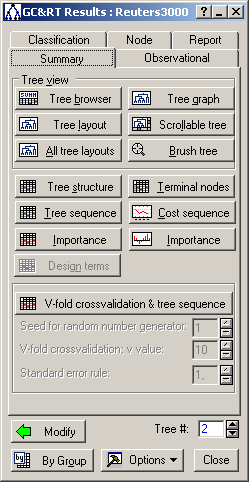
\includegraphics[height=8cm]
    {inc/31.PNG}

    \caption{31}

    \label{fig:31}
  \end{minipage}
  \begin{minipage}{0.69\textwidth}
    \centering

    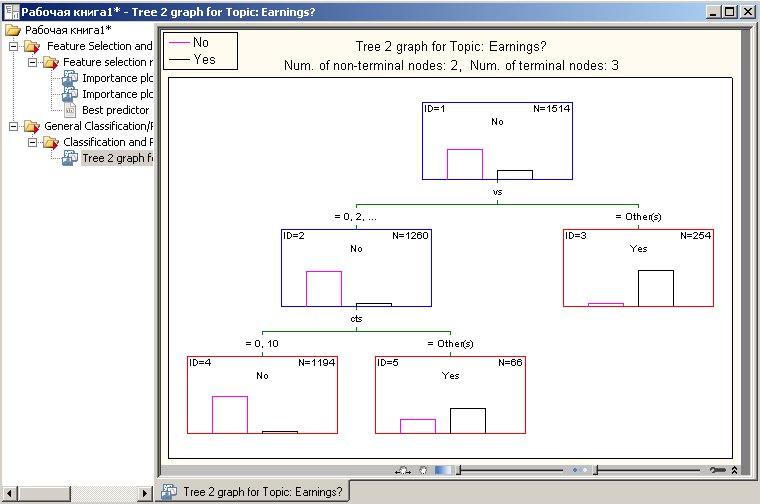
\includegraphics[height=8cm]
    {inc/32.PNG}

    \caption{32}

    \label{fig:32}
  \end{minipage}
\end{figure}

> GC\&RT Results : Reuters3000 \\
> Classification > Sample > Test set \\
> Predicted vs. Observed by classes \\

Результаты на рисункax~\ref{fig:33}, \ref{fig:34}.

\begin{figure}[!h]
  \centering

  \begin{minipage}{0.29\textwidth}
    \centering

    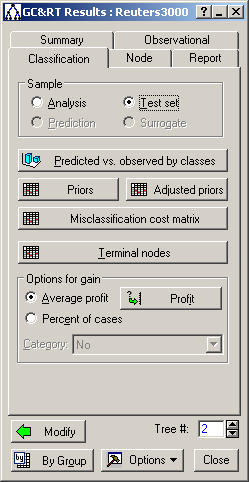
\includegraphics[height=5cm]
    {inc/33.PNG}

    \caption{33}

    \label{fig:33}
  \end{minipage}
  \begin{minipage}{0.69\textwidth}
    \centering

    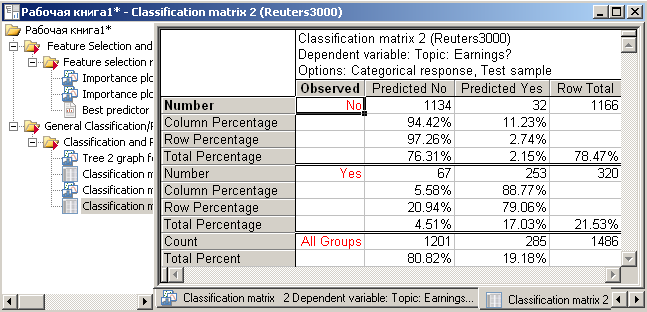
\includegraphics[height=5cm]
    {inc/34.PNG}

    \caption{34}

    \label{fig:34}
  \end{minipage}
\end{figure}

\newpage

\begin{center}
  \textbf{Интерпретация результатов}
\end{center}

Из матрицы классификации можно сделать следующие выводы.

\begin{itemize}
  \item количество случаев, когда классификация с ответом No (Predicted No) правильная,
  т.е. соответствует эталонам с ответом No (Observed No) - \underline{1134};
  \item количество случаев, когда классификация с ответом Yes (Predicted Yes) правильная,
  т.е. соответствует эталонам с ответом Yes (Observed Yes) - \underline{253};
  \item общее количество случаев успешной классификации (прогноза) - \underline{$1134+253=1387$};
  \item количество случаев, когда классификация с ответом No (Predicted No)
  неправильная, т.е. соответствует эталонам с ответом Yes (Observed Yes) - ошибка 1
  рода - \underline{67};
  \item количество случаев, когда классификация с ответом Yes (Predicted Yes)
  неправильная, т.е. соответствует эталонам с ответом No (Observed No) - ошибка 2
  рода - \underline{32};
  \item общее количество случаев неуспешной классификации (прогноза) - \underline{$67+32=99$};
  \item общее количество случаев (элементов выборки, Count) - \underline{1486}.
\end{itemize}


Отсюда можно рассчитать точность прогноза:
$$
P = (1387 / 1486) * 100\% \approx 93,34\%
$$

Общая ошибка прогноза:

$$
P = (99 / 1486) * 100\% \approx 6,66\%
$$

Ошибка прогноза 1 рода:
$$
P = (67 / 1486) * 100\% \approx 4,51\%
$$

Ошибка прогноза 2 рода:
$$
P = (32 / 1486) * 100\% \approx 2,15\%
$$

\newpage

\begin{center}
  \textbf{Вариант 5}
\end{center}

Удаляю папку <<Statistica 10 RUS>> (тут временные файлы portable программы).

Запускаю Ststatistica\_10\_ru\_portable.exe.

\begin{center}
  \textbf{Определение анализа}
\end{center}

Главная > Открыть > <<Reuters for vars.xlsx>> > Открыть \\
> Импортировать выбранный лист в Таблицу данных > Var5 > OK \\
> Имена переменных из первой строки (uncheked) \\
> Имена наблюдений из первого столбца (unchecked) \\
> OK > Импорт, как текстовые метки (3 раза) \\

1 Пер1 > Имя > File Name > OK

2 Пер2 > Имя > Topic: Earnings? > OK

3 Пер3 > Имя > Training > OK

Результаты на рисунке~\ref{fig:var5_1}.

\begin{figure}[!h]
  \centering

  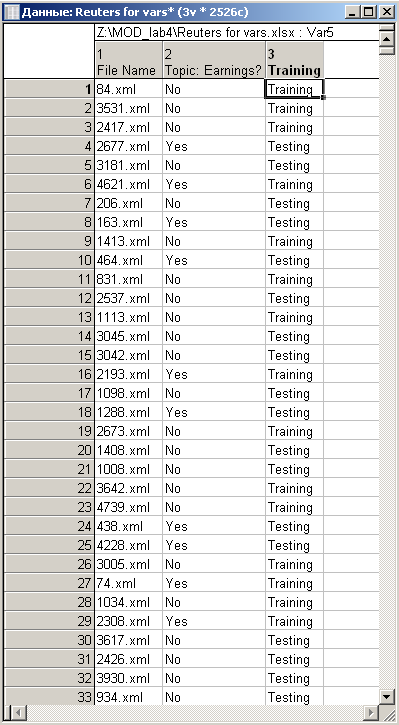
\includegraphics[height=14cm]
  {inc/var5/1.PNG}

  \caption{1}

  \label{fig:var5_1}
\end{figure}

\newpage

Добыча Данных > Добыча текста > Quick \\
> Retrieve text from: > Files \\
> Browse document > Добавить > 1.xml > Shift > 5000.xml > Открыть > OK \\
> Paths in spreadsheet > Document paths \\
> 1 – File Name > OK \\

Результаты на рисункax~\ref{fig:var5_2}, \ref{fig:var5_3}, \ref{fig:var5_4}.

\begin{figure}[!h]
  \centering

  \begin{minipage}{0.32\textwidth}
    \centering

    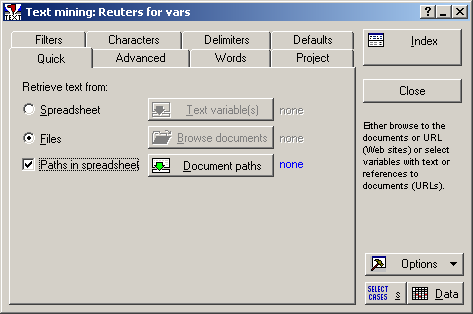
\includegraphics[height=4cm]
    {inc/var5/2.PNG}

    \caption{2}

    \label{fig:var5_2}
  \end{minipage}
  \begin{minipage}{0.32\textwidth}
    \centering

    \includegraphics[height=4cm]
    {inc/var5/3.PNG}

    \caption{3}

    \label{fig:var5_3}
  \end{minipage}
  \begin{minipage}{0.32\textwidth}
    \centering

    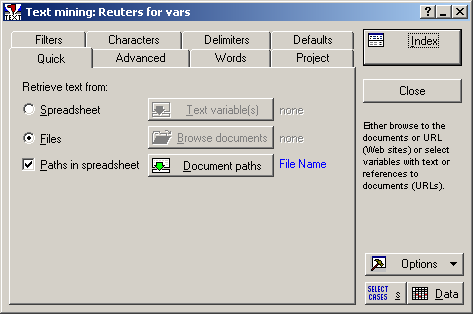
\includegraphics[height=4cm]
    {inc/var5/4.PNG}

    \caption{4}

    \label{fig:var5_4}
  \end{minipage}
\end{figure}


> Advanced > Stemming language > English \\
> \% files where word occurs: > Min > 3 \\
> Words > Stop words (discarded, excluded from indexing) > Select > EnglishStopList,txt > Открыть \\

Результаты на рисункax~\ref{fig:var5_5}, \ref{fig:var5_6}, \ref{fig:var5_7}, \ref{fig:var5_8}.

\begin{figure}[!h]
  \centering

  \begin{minipage}{0.49\textwidth}
    \centering

    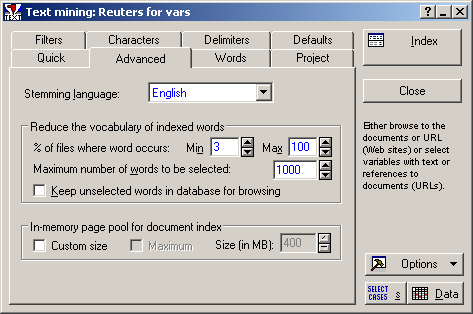
\includegraphics[height=5cm]
    {inc/var5/5.PNG}

    \caption{5}

    \label{fig:var5_5}
  \end{minipage}
  \begin{minipage}{0.49\textwidth}
    \centering

    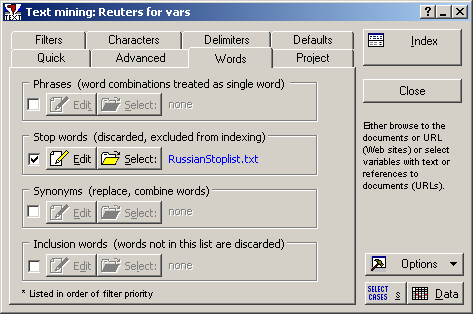
\includegraphics[height=5cm]
    {inc/var5/6.PNG}

    \caption{6}

    \label{fig:var5_6}
  \end{minipage}
\end{figure}

\begin{figure}[!h]
  \centering

  \begin{minipage}{0.49\textwidth}
    \centering

    \includegraphics[height=4cm]
    {inc/var5/7.PNG}

    \caption{7}

    \label{fig:var5_7}
  \end{minipage}
  \begin{minipage}{0.49\textwidth}
    \centering

    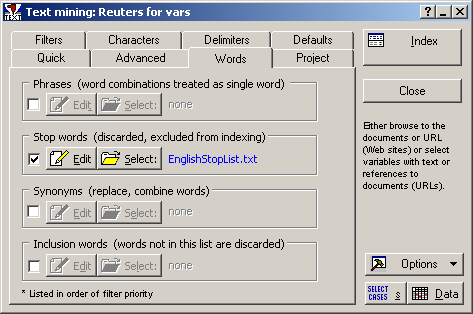
\includegraphics[height=4cm]
    {inc/var5/8.PNG}

    \caption{8}

    \label{fig:var5_8}
  \end{minipage}
\end{figure}

\newpage

\begin{center}
  \textbf{Выполнение анализа данных}
\end{center}

> Index > Да

Результаты на рисунке~\ref{fig:var5_9}.

\begin{figure}[!h]
  \centering

  \includegraphics[height=2cm]
  {inc/var5/9.PNG}

  \caption{9}

  \label{fig:var5_9}
\end{figure}

\begin{center}
  \textbf{Сохранения извлеченных частот слов во входной файл}
\end{center}

> Save results > Ammount > 356 > Append empty variables > OK \\
> Save results > Write back current results (to selected variables) \\

Результаты на рисункax~\ref{fig:var5_10}, \ref{fig:var5_11}, \ref{fig:var5_12}.

\begin{figure}[!h]
  \centering

  \begin{minipage}{0.49\textwidth}
    \centering

    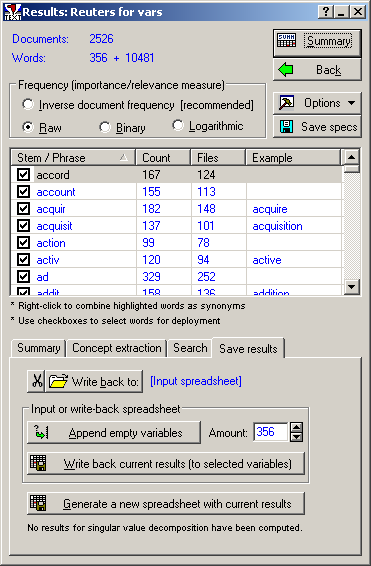
\includegraphics[height=7cm]
    {inc/var5/10.PNG}

    \caption{10}

    \label{fig:var5_10}
  \end{minipage}
  \begin{minipage}{0.49\textwidth}
    \centering

    \includegraphics[height=2cm]
    {inc/var5/11.PNG}

    \caption{11}

    \label{fig:var5_11}
  \end{minipage}
\end{figure}

\begin{figure}[p!h]
  \centering

  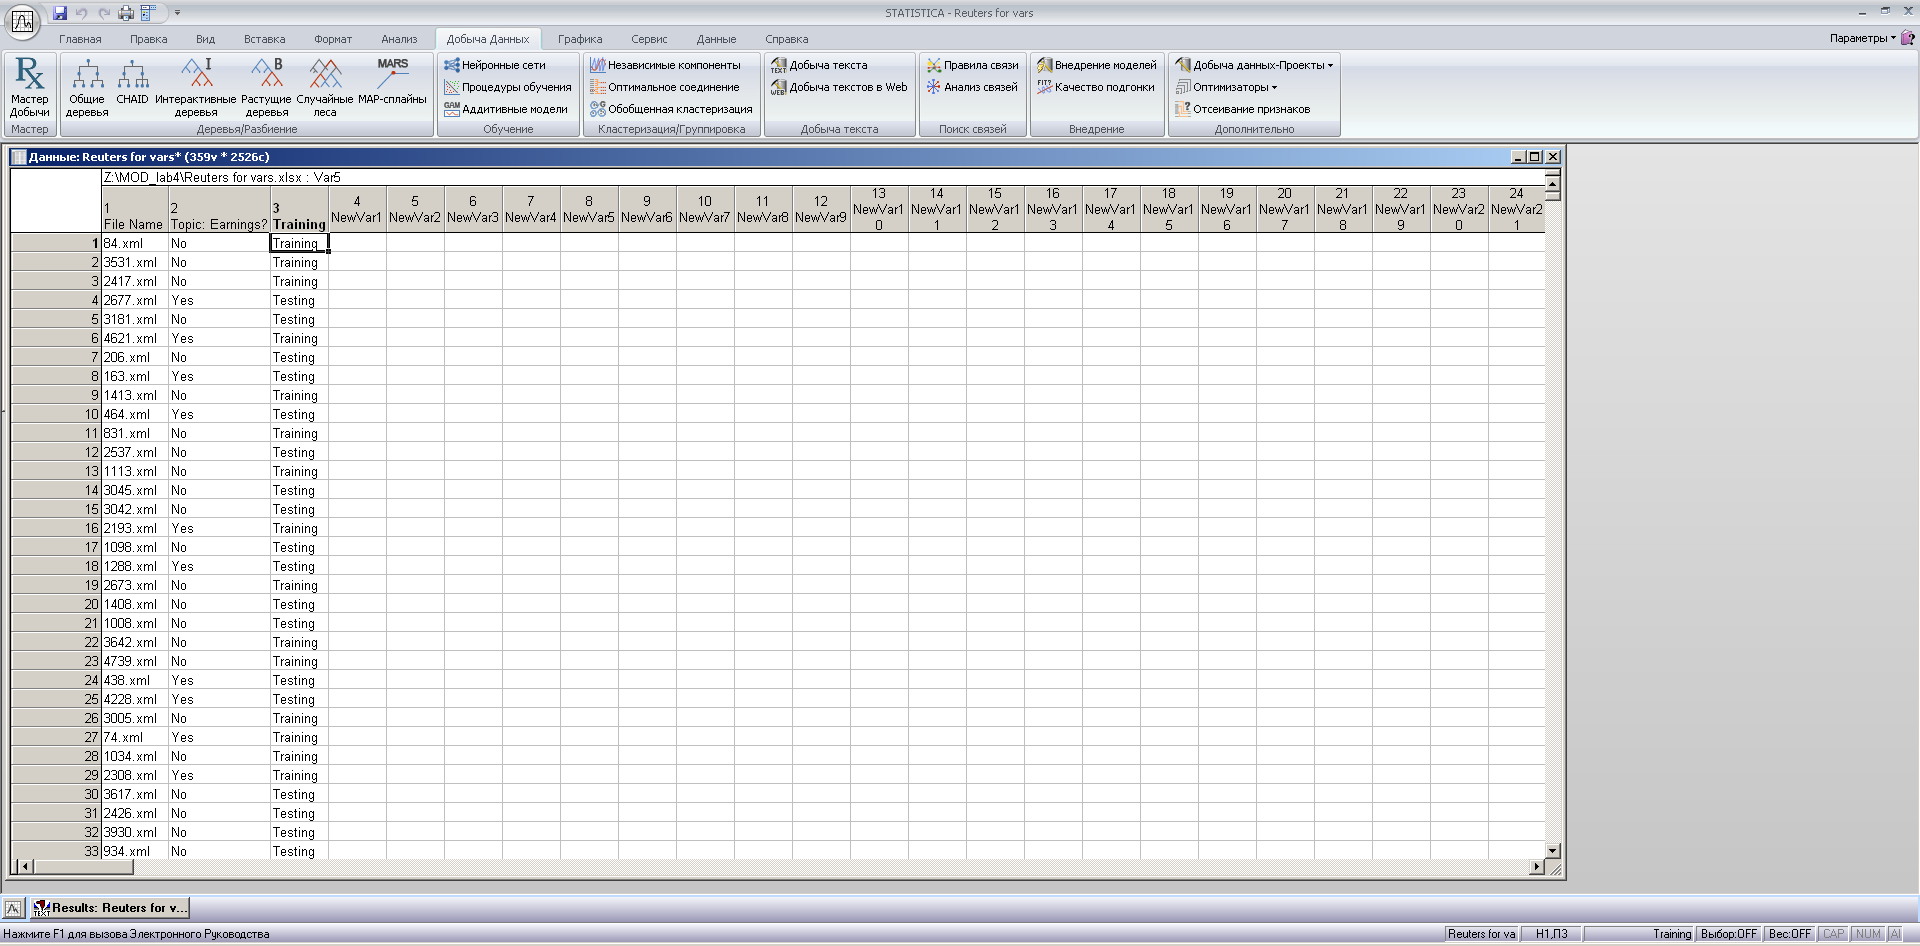
\includegraphics[width=17cm]
  {inc/var5/12.PNG}

  \caption{12}

  \label{fig:var5_12}
\end{figure}


> Statistics > account > Shift > york \\
> Variables > 4 - NewVar1 > Shift > 359 — NewVar356 \\
> Присвоить > OK \\

Результаты на рисункax~\ref{fig:var5_13}, \ref{fig:var5_14}, \ref{fig:var5_15}.

\begin{figure}[p!h]
  \centering

  \begin{minipage}{0.49\textwidth}
    \centering

    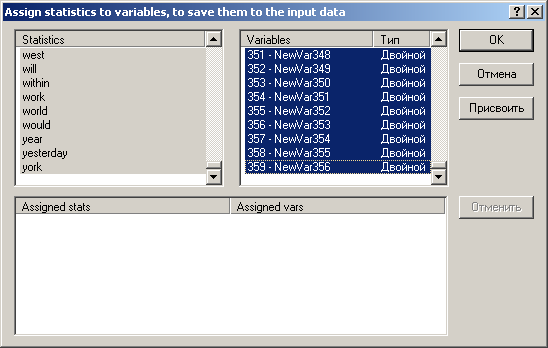
\includegraphics[height=5cm]
    {inc/var5/13.PNG}

    \caption{13}

    \label{fig:var5_13}
  \end{minipage}
  \begin{minipage}{0.49\textwidth}
    \centering

    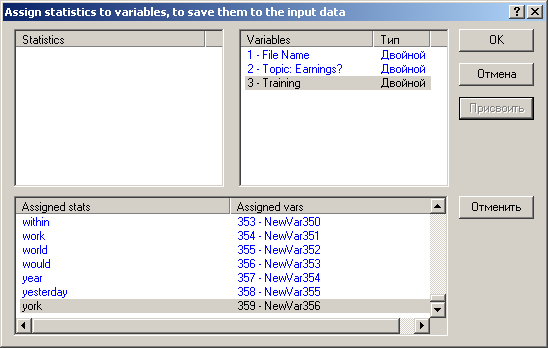
\includegraphics[height=5cm]
    {inc/var5/14.PNG}

    \caption{14}

    \label{fig:var5_14}
  \end{minipage}
\end{figure}

\begin{figure}[p!h]
  \centering

  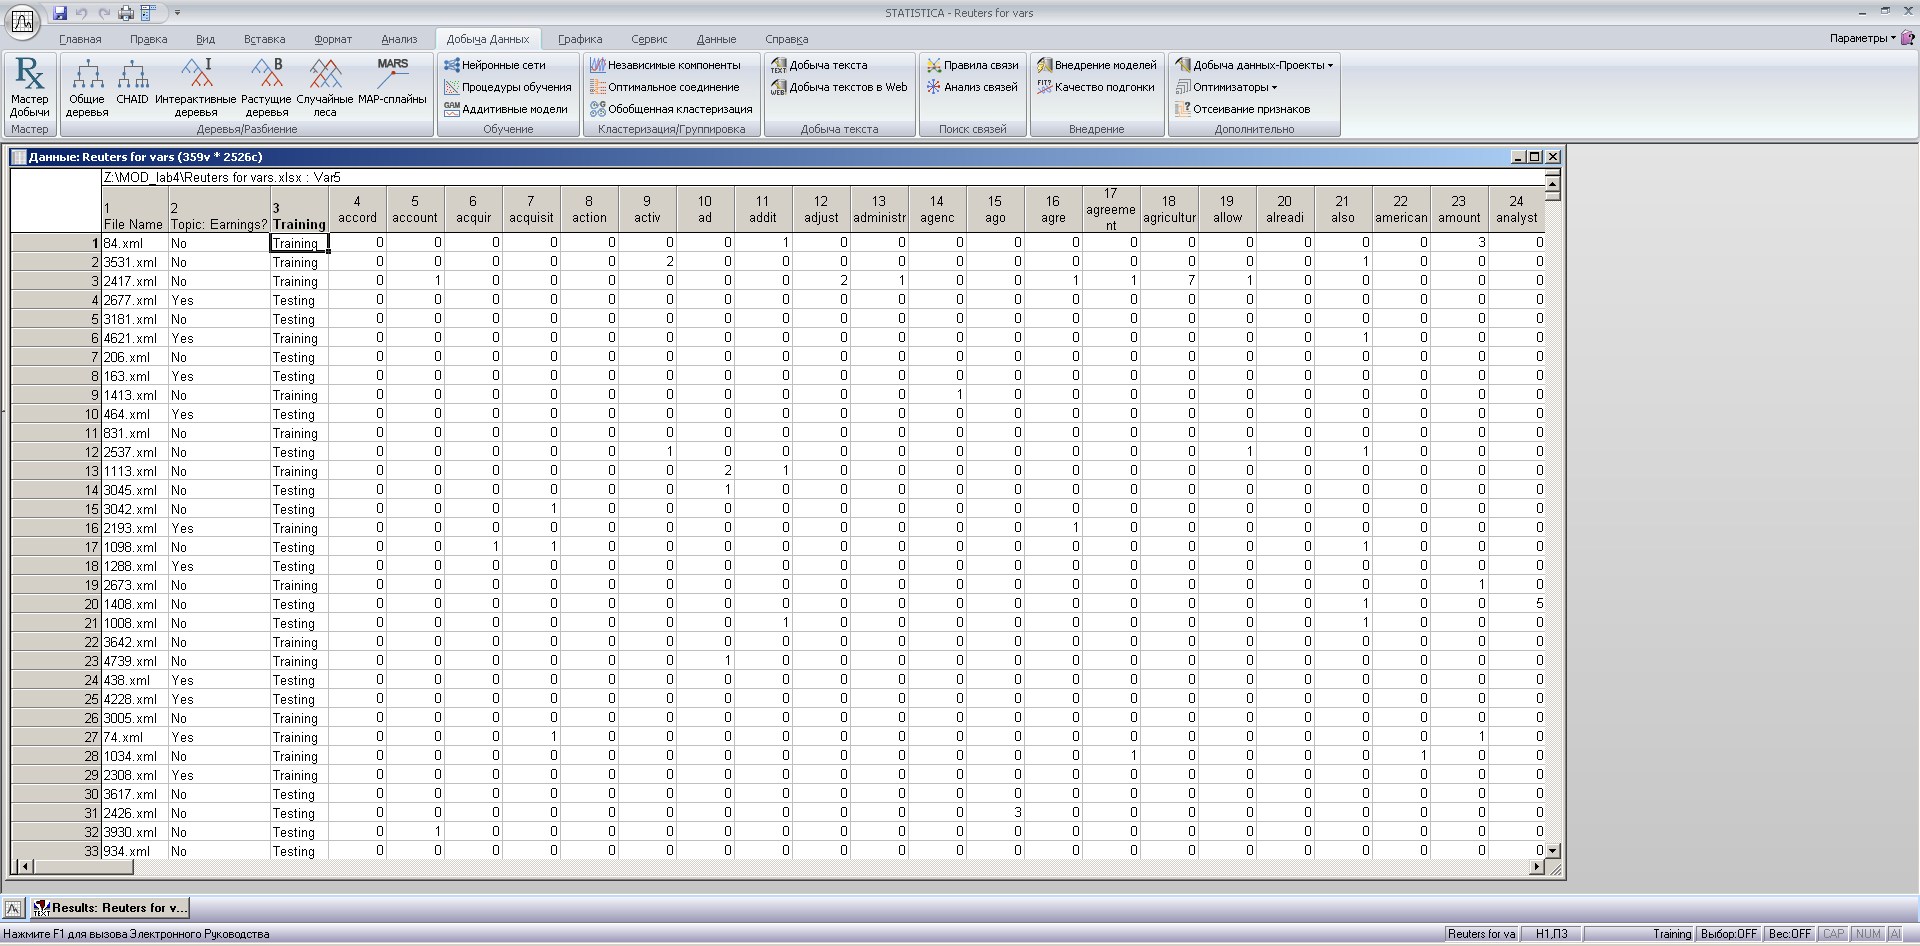
\includegraphics[width=17cm]
  {inc/var5/15.PNG}

  \caption{15}

  \label{fig:var5_15}
\end{figure}

\newpage

\begin{center}
  \textbf{Первоначальный выбор функций}
\end{center}

> Добыча Данных > Отсеивание признаков > Variables \\
> Dependent, categorical > 2 — Topic: Earnings \\
> Predictors; contimuous > 4 — accord > Shift > 359-york \\
> OK > OK \\

Результаты на рисункax~\ref{fig:var5_16}, \ref{fig:var5_17}, \ref{fig:var5_18}.

\begin{figure}[!h]
  \centering

  \begin{minipage}{0.22\textwidth}
    \centering

    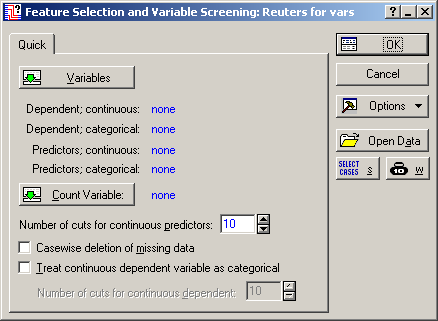
\includegraphics[height=3cm]
    {inc/var5/16.PNG}

    \caption{16}

    \label{fig:var5_16}
  \end{minipage}
  \begin{minipage}{0.52\textwidth}
    \centering

    \includegraphics[height=4cm]
    {inc/var5/17.PNG}

    \caption{17}

    \label{fig:var5_17}
  \end{minipage}
  \begin{minipage}{0.22\textwidth}
    \centering

    \includegraphics[height=3cm]
    {inc/var5/18.PNG}

    \caption{18}

    \label{fig:var5_18}
  \end{minipage}
\end{figure}

> Quick > Display > 50 > Histogram of importance for best k predictors \\

Результаты на рисункax~\ref{fig:var5_19}, \ref{fig:var5_20}.

\begin{figure}[!h]
  \centering

  \begin{minipage}{0.29\textwidth}
    \centering

    \includegraphics[height=4cm]
    {inc/var5/19.PNG}

    \caption{19}

    \label{fig:var5_19}
  \end{minipage}
  \begin{minipage}{0.69\textwidth}
    \centering

    \includegraphics[height=6cm]
    {inc/var5/20.PNG}

    \caption{20}

    \label{fig:var5_20}
  \end{minipage}
\end{figure}

FSL Results : Reuters for vars > Quick > Display > 20 \\
> Histogram of importance for best k predictors

Результаты на рисункax~\ref{fig:var5_21}, \ref{fig:var5_22}.

\begin{figure}[!h]
  \centering

  \begin{minipage}{0.29\textwidth}
    \centering

    \includegraphics[height=4cm]
    {inc/var5/21.PNG}

    \caption{21}

    \label{fig:var5_21}
  \end{minipage}
  \begin{minipage}{0.69\textwidth}
    \centering

    \includegraphics[height=6cm]
    {inc/var5/22.PNG}

    \caption{22}

    \label{fig:var5_22}
  \end{minipage}
\end{figure}

\newpage

FSL Results : Reuters for vars > Quick > Report of best k predictors (features) \\

Результаты на рисунке~\ref{fig:var5_23}.

Копируем номера переменных:
346 87 309 221 292 286 196 261 226 105 211 310 36 268 256 275 106 235 123 352

\begin{figure}[!h]
  \centering

  \includegraphics[height=6cm]
  {inc/var5/23.PNG}

  \caption{23}

  \label{fig:var5_23}
\end{figure}

Вид > Класическое Меню \\
> Добыча Данных > Общие деревья классификаии и регрессии \\
> Quick \\
> Type of analysis > Standart C\&RT \\
> Specification method > Quick specs dialog \\
> OK \\

Результат на рисунке~\ref{fig:24}.

\begin{figure}[!h]
  \centering

  \includegraphics[height=4cm]
  {inc/var5/24.PNG}

  \caption{24}

  \label{fig:var5_24}
\end{figure}

\newpage

> Quick > Categorical response (categorical dependent variable) (checked) \\
> Variables \\
> Depend > 2 — Topic: Earnings? \\
> Continuous pred\\
> 346 87 309 221 292 286 196 261 226 105 211 310 36 268 256 275 106 235 123 352 > OK\\

Результаты на рисункax~\ref{fig:var5_25}, \ref{fig:var5_26}.

\begin{figure}[!h]
  \centering

  \begin{minipage}{0.29\textwidth}
    \centering

    \includegraphics[height=4cm]
    {inc/var5/25.PNG}

    \caption{25}

    \label{fig:var5_25}
  \end{minipage}
  \begin{minipage}{0.69\textwidth}
    \centering

    \includegraphics[height=4.5cm]
    {inc/var5/26.PNG}

    \caption{26}

    \label{fig:var5_26}
  \end{minipage}
\end{figure}

> Validation > V-fold cross-validation \\
> Test sample \\
> Status > on \\
> Sample Identifier Variable > 3 — Training > OK \\
> OK > OK \\

Результаты на рисункax~\ref{fig:var5_27}, \ref{fig:var5_28}, \ref{fig:var5_29}, \ref{fig:var5_30}.

\begin{figure}[!h]
  \centering

  \begin{minipage}{0.49\textwidth}
    \centering

    \includegraphics[height=4cm]
    {inc/var5/27.PNG}

    \caption{27}

    \label{fig:var5_27}
  \end{minipage}
  \begin{minipage}{0.49\textwidth}
    \centering

    \includegraphics[height=4cm]
    {inc/var5/28.PNG}

    \caption{28}

    \label{fig:var5_28}
  \end{minipage}
\end{figure}

\begin{figure}[!h]
  \centering

  \begin{minipage}{0.49\textwidth}
    \centering

    \includegraphics[height=4cm]
    {inc/var5/29.PNG}

    \caption{29}

    \label{fig:var5_29}
  \end{minipage}
  \begin{minipage}{0.49\textwidth}
    \centering

    \includegraphics[height=4cm]
    {inc/var5/30.PNG}

    \caption{30}

    \label{fig:var5_30}
  \end{minipage}
\end{figure}

\newpage

> Summary > Tree graph

Результаты на рисункax~\ref{fig:var5_31}, \ref{fig:var5_32}.

\begin{figure}[!h]
  \centering

  \begin{minipage}{0.29\textwidth}
    \centering

    \includegraphics[height=8cm]
    {inc/var5/31.PNG}

    \caption{31}

    \label{fig:var5_31}
  \end{minipage}
  \begin{minipage}{0.69\textwidth}
    \centering

    \includegraphics[height=8cm]
    {inc/var5/32.PNG}

    \caption{32}

    \label{fig:var5_32}
  \end{minipage}
\end{figure}

> GC\&RT Results : Reuters for vars \\
> Classification > Sample > Test set \\
> Predicted vs. Observed by classes \\

Результаты на рисункax~\ref{fig:var5_33}, \ref{fig:var5_34}.

\begin{figure}[!h]
  \centering

  \begin{minipage}{0.29\textwidth}
    \centering

    \includegraphics[height=5cm]
    {inc/var5/33.PNG}

    \caption{33}

    \label{fig:var5_33}
  \end{minipage}
  \begin{minipage}{0.69\textwidth}
    \centering

    \includegraphics[height=5cm]
    {inc/var5/34.PNG}

    \caption{34}

    \label{fig:var5_34}
  \end{minipage}
\end{figure}

\newpage

\begin{center}
  \textbf{Интерпретация результатов}
\end{center}

Из матрицы классификации можно сделать следующие выводы.

\begin{itemize}
  \item количество случаев, когда классификация с ответом No (Predicted No) правильная,
  т.е. соответствует эталонам с ответом No (Observed No) - \underline{997};
  \item количество случаев, когда классификация с ответом Yes (Predicted Yes) правильная,
  т.е. соответствует эталонам с ответом Yes (Observed Yes) - \underline{218};
  \item общее количество случаев успешной классификации (прогноза) - \underline{$997+218=1215$};
  \item количество случаев, когда классификация с ответом No (Predicted No)
  неправильная, т.е. соответствует эталонам с ответом Yes (Observed Yes) - ошибка 1
  рода - \underline{41};
  \item количество случаев, когда классификация с ответом Yes (Predicted Yes)
  неправильная, т.е. соответствует эталонам с ответом No (Observed No) - ошибка 2
  рода - \underline{31};
  \item общее количество случаев неуспешной классификации (прогноза) - \underline{$41+31=72$};
  \item общее количество случаев (элементов выборки, Count) - \underline{1287}.
\end{itemize}


Отсюда можно рассчитать точность прогноза:
$$
P = (1215 / 1287) * 100\% \approx 94,41\%
$$

Общая ошибка прогноза:

$$
P = (72 / 1287) * 100\% \approx 5,59\%
$$

Ошибка прогноза 1 рода:
$$
P = (41 / 1287) * 100\% \approx 3,19\%
$$

Ошибка прогноза 2 рода:
$$
P = (31 / 1287) * 100\% \approx 2,41\%
$$

\newpage
